% Options for packages loaded elsewhere
\PassOptionsToPackage{unicode}{hyperref}
\PassOptionsToPackage{hyphens}{url}
\PassOptionsToPackage{dvipsnames,svgnames,x11names}{xcolor}
%
\documentclass[
  10pt,
]{article}

\usepackage{amsmath,amssymb}
\usepackage{setspace}
\usepackage{iftex}
\ifPDFTeX
  \usepackage[T1]{fontenc}
  \usepackage[utf8]{inputenc}
  \usepackage{textcomp} % provide euro and other symbols
\else % if luatex or xetex
  \usepackage{unicode-math}
  \defaultfontfeatures{Scale=MatchLowercase}
  \defaultfontfeatures[\rmfamily]{Ligatures=TeX,Scale=1}
\fi
\usepackage{lmodern}
\ifPDFTeX\else  
    % xetex/luatex font selection
    \setmainfont[]{Book Antiqua}
    \setsansfont[]{Book Antiqua}
\fi
% Use upquote if available, for straight quotes in verbatim environments
\IfFileExists{upquote.sty}{\usepackage{upquote}}{}
\IfFileExists{microtype.sty}{% use microtype if available
  \usepackage[]{microtype}
  \UseMicrotypeSet[protrusion]{basicmath} % disable protrusion for tt fonts
}{}
\makeatletter
\@ifundefined{KOMAClassName}{% if non-KOMA class
  \IfFileExists{parskip.sty}{%
    \usepackage{parskip}
  }{% else
    \setlength{\parindent}{0pt}
    \setlength{\parskip}{6pt plus 2pt minus 1pt}}
}{% if KOMA class
  \KOMAoptions{parskip=half}}
\makeatother
\usepackage{xcolor}
\usepackage[top=2.54cm,bottom=2.54cm,left=3.17cm,right=3.17cm]{geometry}
\setlength{\emergencystretch}{3em} % prevent overfull lines
\setcounter{secnumdepth}{5}
% Make \paragraph and \subparagraph free-standing
\makeatletter
\ifx\paragraph\undefined\else
  \let\oldparagraph\paragraph
  \renewcommand{\paragraph}{
    \@ifstar
      \xxxParagraphStar
      \xxxParagraphNoStar
  }
  \newcommand{\xxxParagraphStar}[1]{\oldparagraph*{#1}\mbox{}}
  \newcommand{\xxxParagraphNoStar}[1]{\oldparagraph{#1}\mbox{}}
\fi
\ifx\subparagraph\undefined\else
  \let\oldsubparagraph\subparagraph
  \renewcommand{\subparagraph}{
    \@ifstar
      \xxxSubParagraphStar
      \xxxSubParagraphNoStar
  }
  \newcommand{\xxxSubParagraphStar}[1]{\oldsubparagraph*{#1}\mbox{}}
  \newcommand{\xxxSubParagraphNoStar}[1]{\oldsubparagraph{#1}\mbox{}}
\fi
\makeatother


\providecommand{\tightlist}{%
  \setlength{\itemsep}{0pt}\setlength{\parskip}{0pt}}\usepackage{longtable,booktabs,array}
\usepackage{calc} % for calculating minipage widths
% Correct order of tables after \paragraph or \subparagraph
\usepackage{etoolbox}
\makeatletter
\patchcmd\longtable{\par}{\if@noskipsec\mbox{}\fi\par}{}{}
\makeatother
% Allow footnotes in longtable head/foot
\IfFileExists{footnotehyper.sty}{\usepackage{footnotehyper}}{\usepackage{footnote}}
\makesavenoteenv{longtable}
\usepackage{graphicx}
\makeatletter
\newsavebox\pandoc@box
\newcommand*\pandocbounded[1]{% scales image to fit in text height/width
  \sbox\pandoc@box{#1}%
  \Gscale@div\@tempa{\textheight}{\dimexpr\ht\pandoc@box+\dp\pandoc@box\relax}%
  \Gscale@div\@tempb{\linewidth}{\wd\pandoc@box}%
  \ifdim\@tempb\p@<\@tempa\p@\let\@tempa\@tempb\fi% select the smaller of both
  \ifdim\@tempa\p@<\p@\scalebox{\@tempa}{\usebox\pandoc@box}%
  \else\usebox{\pandoc@box}%
  \fi%
}
% Set default figure placement to htbp
\def\fps@figure{htbp}
\makeatother
% definitions for citeproc citations
\NewDocumentCommand\citeproctext{}{}
\NewDocumentCommand\citeproc{mm}{%
  \begingroup\def\citeproctext{#2}\cite{#1}\endgroup}
\makeatletter
 % allow citations to break across lines
 \let\@cite@ofmt\@firstofone
 % avoid brackets around text for \cite:
 \def\@biblabel#1{}
 \def\@cite#1#2{{#1\if@tempswa , #2\fi}}
\makeatother
\newlength{\cslhangindent}
\setlength{\cslhangindent}{1.5em}
\newlength{\csllabelwidth}
\setlength{\csllabelwidth}{3em}
\newenvironment{CSLReferences}[2] % #1 hanging-indent, #2 entry-spacing
 {\begin{list}{}{%
  \setlength{\itemindent}{0pt}
  \setlength{\leftmargin}{0pt}
  \setlength{\parsep}{0pt}
  % turn on hanging indent if param 1 is 1
  \ifodd #1
   \setlength{\leftmargin}{\cslhangindent}
   \setlength{\itemindent}{-1\cslhangindent}
  \fi
  % set entry spacing
  \setlength{\itemsep}{#2\baselineskip}}}
 {\end{list}}
\usepackage{calc}
\newcommand{\CSLBlock}[1]{\hfill\break\parbox[t]{\linewidth}{\strut\ignorespaces#1\strut}}
\newcommand{\CSLLeftMargin}[1]{\parbox[t]{\csllabelwidth}{\strut#1\strut}}
\newcommand{\CSLRightInline}[1]{\parbox[t]{\linewidth - \csllabelwidth}{\strut#1\strut}}
\newcommand{\CSLIndent}[1]{\hspace{\cslhangindent}#1}

\usepackage{booktabs}
\usepackage{caption}
\usepackage{longtable}
\usepackage{colortbl}
\usepackage{array}
\usepackage{anyfontsize}
\usepackage{multirow}
\usepackage{float}
\usepackage{caption}
\usepackage{pdfpages}
\usepackage{fancyhdr}
\usepackage{graphicx}
\usepackage{booktabs}
\usepackage{longtable}
\usepackage{array}
\usepackage{multirow}
\usepackage{xcolor}
\definecolor{bleuunicef}{HTML}{1CABE2}
\definecolor{bleuNuit}{HTML}{374EA2}
\captionsetup{font=small, labelfont=bf}
\pagestyle{fancy}
\fancyhf{}
\fancyhead[L]{\small\textit{Nigeria GHS Panel W4 (2018-2019)}}
\fancyhead[R]{\small\textit{Profil démographique des ménages}}
\fancyfoot[C]{\thepage}
\renewcommand{\headrulewidth}{0.4pt}
\setcounter{page}{1}
\AtBeginDocument{\let\maketitle\relax}
\makeatletter
\@ifpackageloaded{tcolorbox}{}{\usepackage[skins,breakable]{tcolorbox}}
\@ifpackageloaded{fontawesome5}{}{\usepackage{fontawesome5}}
\definecolor{quarto-callout-color}{HTML}{909090}
\definecolor{quarto-callout-note-color}{HTML}{0758E5}
\definecolor{quarto-callout-important-color}{HTML}{CC1914}
\definecolor{quarto-callout-warning-color}{HTML}{EB9113}
\definecolor{quarto-callout-tip-color}{HTML}{00A047}
\definecolor{quarto-callout-caution-color}{HTML}{FC5300}
\definecolor{quarto-callout-color-frame}{HTML}{acacac}
\definecolor{quarto-callout-note-color-frame}{HTML}{4582ec}
\definecolor{quarto-callout-important-color-frame}{HTML}{d9534f}
\definecolor{quarto-callout-warning-color-frame}{HTML}{f0ad4e}
\definecolor{quarto-callout-tip-color-frame}{HTML}{02b875}
\definecolor{quarto-callout-caution-color-frame}{HTML}{fd7e14}
\makeatother
\makeatletter
\@ifpackageloaded{caption}{}{\usepackage{caption}}
\AtBeginDocument{%
\ifdefined\contentsname
  \renewcommand*\contentsname{Table des matières}
\else
  \newcommand\contentsname{Table des matières}
\fi
\ifdefined\listfigurename
  \renewcommand*\listfigurename{Liste des Figures}
\else
  \newcommand\listfigurename{Liste des Figures}
\fi
\ifdefined\listtablename
  \renewcommand*\listtablename{Liste des Tables}
\else
  \newcommand\listtablename{Liste des Tables}
\fi
\ifdefined\figurename
  \renewcommand*\figurename{Figure}
\else
  \newcommand\figurename{Figure}
\fi
\ifdefined\tablename
  \renewcommand*\tablename{Table}
\else
  \newcommand\tablename{Table}
\fi
}
\@ifpackageloaded{float}{}{\usepackage{float}}
\floatstyle{ruled}
\@ifundefined{c@chapter}{\newfloat{codelisting}{h}{lop}}{\newfloat{codelisting}{h}{lop}[chapter]}
\floatname{codelisting}{Listing}
\newcommand*\listoflistings{\listof{codelisting}{Liste des Listings}}
\makeatother
\makeatletter
\makeatother
\makeatletter
\@ifpackageloaded{caption}{}{\usepackage{caption}}
\@ifpackageloaded{subcaption}{}{\usepackage{subcaption}}
\makeatother

\ifLuaTeX
\usepackage[bidi=basic]{babel}
\else
\usepackage[bidi=default]{babel}
\fi
\babelprovide[main,import]{french}
\ifPDFTeX
\else
\babelfont{rm}[]{Book Antiqua}
\fi
% get rid of language-specific shorthands (see #6817):
\let\LanguageShortHands\languageshorthands
\def\languageshorthands#1{}
\usepackage{bookmark}

\IfFileExists{xurl.sty}{\usepackage{xurl}}{} % add URL line breaks if available
\urlstyle{same} % disable monospaced font for URLs
\hypersetup{
  pdftitle={Profil démographique des ménages nigérians},
  pdfauthor={Keita L.; Nkwa Tsamo L.},
  pdflang={fr},
  colorlinks=true,
  linkcolor={blue},
  filecolor={Maroon},
  citecolor={Blue},
  urlcolor={Blue},
  pdfcreator={LaTeX via pandoc}}


\title{Profil démographique des ménages nigérians}
\usepackage{etoolbox}
\makeatletter
\providecommand{\subtitle}[1]{% add subtitle to \maketitle
  \apptocmd{\@title}{\par {\large #1 \par}}{}{}
}
\makeatother
\subtitle{Analyse du Nigeria General Household Survey Panel Wave 4
(2018-2019)}
\author{Keita L. \and Nkwa Tsamo L.}
\date{17 mars 2026}

\begin{document}
\maketitle

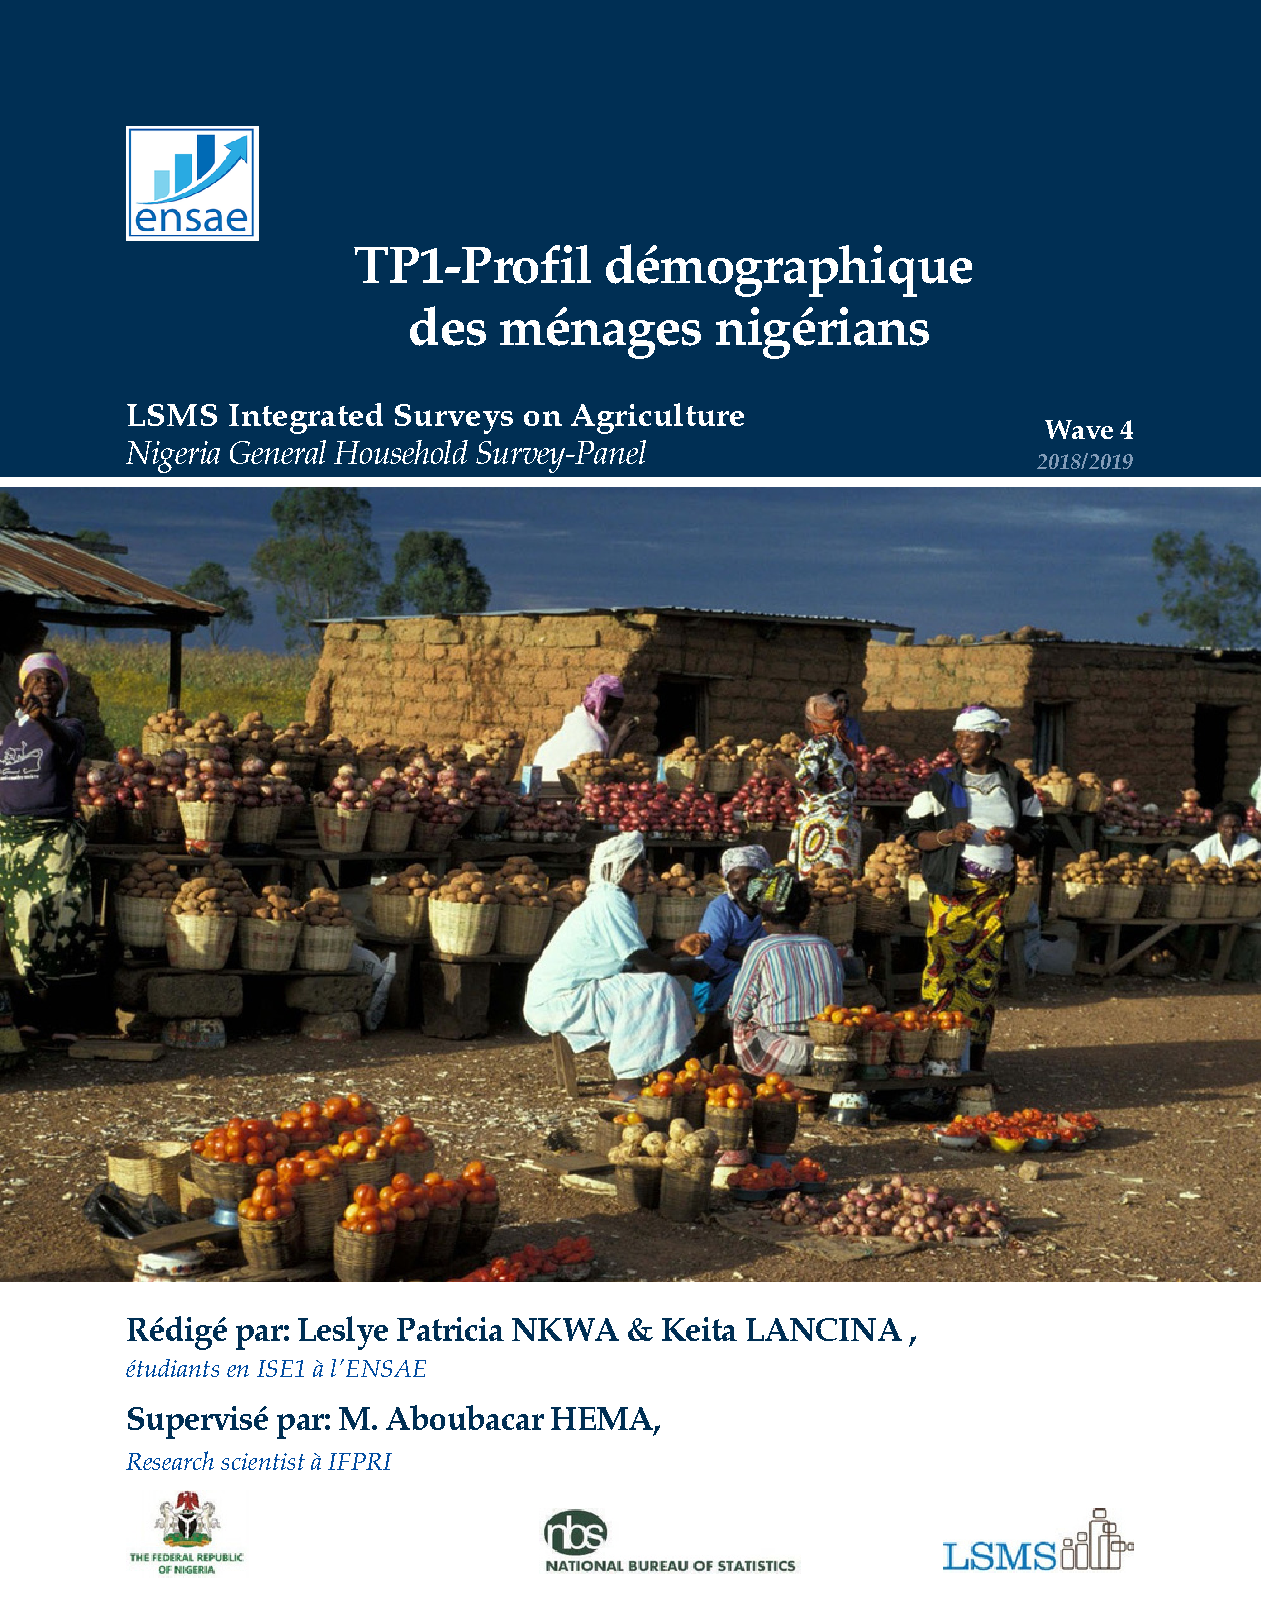
\includepdf[pages=1]{cover_canva.pdf}
\newpage

\renewcommand*\contentsname{Table des matières}
{
\hypersetup{linkcolor=}
\setcounter{tocdepth}{3}
\tableofcontents
}

\setstretch{1.7}
\newpage{}

\section*{Messages clés}\label{messages-cluxe9s}
\addcontentsline{toc}{section}{Messages clés}

\begin{tcolorbox}[enhanced jigsaw, breakable, bottomrule=.15mm, colbacktitle=quarto-callout-note-color!10!white, colback=white, titlerule=0mm, bottomtitle=1mm, toptitle=1mm, opacitybacktitle=0.6, arc=.35mm, opacityback=0, left=2mm, colframe=quarto-callout-note-color-frame, rightrule=.15mm, title={Principaux résultats}, toprule=.15mm, coltitle=black, leftrule=.75mm]

\textbf{Structure démographique}

\begin{itemize}
\item
  La population nigériane est \textbf{très jeune} : âge médian de
  \textbf{18 ans}, reflet d'une fécondité élevée (ISF ≈ 5,3 en 2018, DHS
  Nigeria).
\item
  \textbf{Équilibre des sexes} quasi parfait : 49.8\% d'hommes, 50.2\%
  de femmes.
\end{itemize}

\textbf{Composition des ménages}

\begin{itemize}
\item
  Les \textbf{enfants} représentent \textbf{55.6\%} des membres --- plus
  de la moitié de la population enquêtée.
\item
  Taille médiane des ménages : \textbf{5 membres} (niveau ménage).
\end{itemize}

\textbf{Disparités rural-urbain}

\begin{itemize}
\item
  Les ménages \textbf{ruraux} sont \textbf{plus grands} (médiane = 5)
  que les ménages \textbf{urbains} (médiane = 4).
\item
  La population \textbf{rurale} est \textbf{plus jeune} (médiane = 17
  ans) que la population \textbf{urbaine} (médiane = 20 ans).
\item
  Ces différences sont \textbf{statistiquement significatives} (test de
  Wilcoxon, p \textless{} 0,001) mais d'\textbf{ampleur modeste} (r
  \textless{} 0,15, Cohen 1988).
\end{itemize}

\textbf{Qualité des données}

\begin{itemize}
\tightlist
\item
  4 570 membres non résidents exclus (filtre \texttt{s1q4a\ ==\ 1}). Un
  âge aberrant de 130 ans recodé en NA --- individu conservé.
\item
  45 ménages d'attrition totale identifiés (taux de complétion
  post-harvest : 99,1\%).
\item
  0 doublon sur la clé \texttt{hhid\ +\ indiv}.
\end{itemize}

\end{tcolorbox}

\newpage{}

\section{Introduction}\label{introduction}

\subsection{Contexte}\label{contexte}

Le Nigeria, avec ses 200 millions d'habitants en 2018, est le pays le
plus peuplé d'Afrique (World Bank, 2018). Sa structure démographique se
caractérise par une \textbf{forte fécondité} (Indice Synthétique de
Fécondité ≈ 5,3 enfants par femme) et une \textbf{population très jeune}
(âge médian national de 17,9 ans selon le DHS Nigeria 2018), typique des
pays en \textbf{transition démographique précoce}.

Les ménages nigérians présentent des configurations variées selon le
milieu de résidence (rural/urbain), la zone géopolitique (Nord/Sud), et
le niveau socio-économique. Comprendre cette \textbf{diversité
démographique} est essentiel pour concevoir des \textbf{politiques
publiques ciblées} en éducation, santé, emploi et protection sociale.

\subsection{Objectifs}\label{objectifs}

Cette analyse vise à dresser un \textbf{profil démographique détaillé}
des ménages nigérians à partir du \textbf{Nigeria General Household
Survey Panel Wave 4 (2018-2019)}, en documentant :

\begin{enumerate}
\def\labelenumi{\arabic{enumi}.}
\tightlist
\item
  La \textbf{distribution de l'âge} et sa conformité à une loi normale
  (test de Shapiro-Wilk) ;
\item
  La \textbf{structure par âge et sexe} via une pyramide démographique ;
\item
  La \textbf{composition des ménages} selon le lien de parenté avec le
  chef de ménage ;
\item
  Les \textbf{disparités rural-urbain} de taille de ménage (test de
  Wilcoxon-Mann-Whitney) ;
\item
  Les \textbf{caractéristiques démographiques} stratifiées par milieu de
  résidence (tableau gtsummary).
\end{enumerate}

\subsection{Questions analytiques}\label{questions-analytiques}

\begin{itemize}
\tightlist
\item
  La distribution de l'âge suit-elle une loi normale ?
\item
  Existe-t-il des différences significatives de taille de ménage entre
  milieux rural et urbain ?
\item
  Quelle est l'ampleur de ces différences et quelles en sont les
  implications ?
\end{itemize}

\newpage{}

\section{Données et méthodes}\label{donnuxe9es-et-muxe9thodes}

\subsection{Source des données}\label{source-des-donnuxe9es}

L'analyse repose sur le \textbf{Nigeria General Household Survey Panel
Wave 4} (GHS-Panel W4), collecté entre août 2018 et avril 2019 par le
\textbf{National Bureau of Statistics (NBS)} en collaboration avec la
\textbf{Banque Mondiale} (programme LSMS-ISA, DOI : 10.48529/1hgw-dq47,
version 03 --- octobre 2021).

\subsubsection{Couverture de l'enquête}\label{couverture-de-lenquuxeate}

\begin{itemize}
\tightlist
\item
  \textbf{Ménages dans le fichier Root} : 5 025 (secta\_harvestw4)
\item
  \textbf{Ménages interviewés} : 4 978 (taux de complétion post-harvest
  : 99,1\%)
\item
  \textbf{Membres résidents actifs} : 25 767 (après filtre
  \texttt{s1q4a\ ==\ 1})
\item
  \textbf{Membres non résidents exclus} : 4 570 (partis, décédés, mariés
  hors ménage)
\item
  \textbf{Stratification} : 6 zones géopolitiques, distinction
  rural/urbain
\item
  \textbf{Attrition totale} : 45 ménages non interviewés (refus,
  introuvables, indisponibles)
\end{itemize}

\subsubsection{Fichiers utilisés}\label{fichiers-utilisuxe9s}

\begin{itemize}
\tightlist
\item
  \textbf{sect1\_harvestw4.dta} : roster individuel --- âge, sexe, lien
  de parenté, statut de résidence
\item
  \textbf{secta\_harvestw4.dta} : fichier Root --- poids, géographie,
  résultats d'interview (validation de cohérence)
\end{itemize}

\subsection{Variables analysées}\label{variables-analysuxe9es}

\begin{longtable}[]{@{}
  >{\raggedright\arraybackslash}p{(\linewidth - 4\tabcolsep) * \real{0.1919}}
  >{\raggedright\arraybackslash}p{(\linewidth - 4\tabcolsep) * \real{0.1414}}
  >{\raggedright\arraybackslash}p{(\linewidth - 4\tabcolsep) * \real{0.6667}}@{}}
\caption{Variables clés de
l'analyse}\label{tbl-variables}\tabularnewline
\toprule\noalign{}
\begin{minipage}[b]{\linewidth}\raggedright
Variable
\end{minipage} & \begin{minipage}[b]{\linewidth}\raggedright
Type
\end{minipage} & \begin{minipage}[b]{\linewidth}\raggedright
Codage
\end{minipage} \\
\midrule\noalign{}
\endfirsthead
\toprule\noalign{}
\begin{minipage}[b]{\linewidth}\raggedright
Variable
\end{minipage} & \begin{minipage}[b]{\linewidth}\raggedright
Type
\end{minipage} & \begin{minipage}[b]{\linewidth}\raggedright
Codage
\end{minipage} \\
\midrule\noalign{}
\endhead
\bottomrule\noalign{}
\endlastfoot
\textbf{s1q4} & Continue & Âge en années complètes (0--100, après
correction) \\
\textbf{s1q2} & Catégorielle & Sexe : 1 = Homme, 2 = Femme \\
\textbf{s1q3} & Catégorielle & Lien de parenté (14 modalités, regroupées
en 4) \\
\textbf{sector} & Catégorielle & Milieu : 1 = Urbain, 2 = Rural \\
\textbf{zone} & Catégorielle & Zone géopolitique (6 zones) \\
\textbf{taille\_menage} & Discrète & Nombre de membres actifs par ménage
(agrégée par \texttt{hhid}) \\
\end{longtable}

\subsection{Traitement des données}\label{traitement-des-donnuxe9es}

\subsubsection{Filtrage et nettoyage}\label{filtrage-et-nettoyage}

Les \textbf{membres non résidents} (\texttt{s1q4a\ !=\ 1}) sont exclus
--- ils présentent des valeurs manquantes structurelles sur toutes les
variables démographiques. Un individu présentant un \textbf{âge de 130
ans} (biologiquement impossible, hhid = 169068, South East) a été recodé
en NA ; l'individu est conservé dans l'échantillon.

\subsubsection{Construction des variables
dérivées}\label{construction-des-variables-duxe9rivuxe9es}

\begin{itemize}
\tightlist
\item
  \textbf{sexe} : recodage de \texttt{s1q2} en facteur (``Homme'',
  ``Femme'')
\item
  \textbf{groupe\_age} : classes quinquennales {[}0,5), {[}5,10),
  \ldots, (convention ONU/UNFPA)
\item
  \textbf{milieu} : recodage de \texttt{sector} en facteur (``Urbain'',
  ``Rural'')
\item
  \textbf{parente} : regroupement de \texttt{s1q3} en 4 catégories (Chef
  de ménage, Conjoint(e), Enfant, Autre)
\item
  \textbf{taille\_menage} : comptage des membres actifs par
  \texttt{hhid}, jointure au niveau individu
\end{itemize}

\subsection{Méthodes statistiques}\label{muxe9thodes-statistiques}

\subsubsection{Analyses descriptives}\label{analyses-descriptives}

Statistiques de position et dispersion (moyenne, médiane, quartiles,
écart-type, coefficient de variation), mesures de forme (asymétrie,
aplatissement via \texttt{moments}), intervalles de confiance à 95\% par
la méthode exacte de Clopper-Pearson (\texttt{PropCIs::exactci}).

\subsubsection{Tests statistiques}\label{tests-statistiques}

\textbf{Test de normalité de Shapiro-Wilk} : H₀ = la distribution de
l'âge suit une loi normale. Appliqué sur un échantillon aléatoire de 5
000 individus (contrainte R), graine fixée à 2070.

\textbf{Test de Wilcoxon-Mann-Whitney} : H₀ = les distributions de
taille de ménage sont identiques en rural et urbain. Test non
paramétrique, justifié par le rejet de la normalité. Complété par la
taille d'effet r de rang (\(r = Z / \sqrt{N}\), seuils de Cohen 1988 :
négligeable \textless{} 0,10 ; petit 0,10--0,30 ; moyen 0,30--0,50).

\subsubsection{Outils et
reproductibilité}\label{outils-et-reproductibilituxe9}

Analyses réalisées avec \textbf{R 4.4} (R Core Team, 2024), packages
\texttt{tidyverse} (Wickham et al., 2019), \texttt{gtsummary} (Sjoberg
et al., 2021), \texttt{rstatix} (Kassambara, 2023), \texttt{apyramid}
(Jombart et al., 2021), \texttt{naniar} (Tierney et al., 2021).
Reproductibilité garantie par \texttt{renv} (Ushey \& Wickham, 2024) ---
voir \texttt{renv.lock}.

\newpage{}

\section{Résultats}\label{ruxe9sultats}

\subsection{Distribution de l'âge}\label{distribution-de-luxe2ge}

\subsubsection{Statistiques
descriptives}\label{statistiques-descriptives}

\begin{table}
\caption*{
{\fontsize{9}{11}\selectfont  Statistiques descriptives de l'âge\fontsize{8}{9}\selectfont } \\ 
{\fontsize{8}{9}\selectfont  Nigeria GHS Panel W4 (2018-2019) — Membres actifs\fontsize{8}{9}\selectfont }
} 
\fontsize{8.0pt}{9.0pt}\selectfont
\begin{tabular*}{\linewidth}{@{\extracolsep{\fill}}lr}
\toprule
Statistique & Valeur \\ 
\midrule\addlinespace[2.5pt]
N (valide) & 25 766 \\ 
Moyenne & 24,37 \\ 
Médiane & 18,0 \\ 
Q1 (25e percentile) & 9,0 \\ 
Q3 (75e percentile) & 37,0 \\ 
Écart-type & 19,73 \\ 
CV (\%) & 81,0 \\ 
Minimum & 0 \\ 
Maximum & 100 \\ 
Asymétrie (skewness) & 0,9817 \\ 
Aplatissement (kurtosis) & 3,2138 \\ 
\bottomrule
\end{tabular*}
\begin{minipage}{\linewidth}
\vspace{.05em}
Source : NBS Nigeria / World Bank LSMS-ISA. Calculs des auteurs.\\
\end{minipage}
\end{table}

La population présente un \textbf{âge médian de 18 ans}, nettement
inférieur à la moyenne (24.4 ans). Cet écart de 6.4 ans révèle une
\textbf{asymétrie positive} (skewness = 0.98) : la distribution est
étalée vers les âges élevés. Le \textbf{coefficient de variation} (81\%)
traduit une \textbf{forte hétérogénéité} de la structure par âge.

\subsubsection{Histogramme de la
distribution}\label{histogramme-de-la-distribution}

!{[}Distribution de l'âge des membres actifs des ménages. La classe
\phantomsection\label{fig-hist-age}\href{outputs/figures/fig01_histogramme_age.png}{0,5)
est la plus peuplée, puis l'effectif décroît régulièrement --- profil
typique d'une population à forte fécondité et mortalité élevée aux âges
avancés. Classes quinquennales selon la convention ONU/UNFPA.}

L'histogramme confirme une \textbf{distribution très asymétrique à
droite} : base large (jeunes), sommet étroit (personnes âgées). Ce
profil est caractéristique d'une \textbf{population à fécondité
soutenue} (ISF ≈ 5,3) et d'une \textbf{espérance de vie limitée} (≈ 54
ans au Nigeria en 2018).

\subsubsection{Boîte à moustaches}\label{bouxeete-uxe0-moustaches}

\begin{figure}[H]

\centering{


\includegraphics[width=1\linewidth,height=\textheight,keepaspectratio]{outputs/figures/fig02_boxplot_age.png}

}

\caption{\label{fig-box-age}Boîte à moustaches de l'âge. La médiane (18
ans) est nettement inférieure à la moyenne (24 ans), confirmant
l'asymétrie positive. Les points au-delà de 1,5 × IQR représentent des
individus réellement âgés, non des erreurs, après correction de la
valeur aberrante de 130 ans.}

\end{figure}%

La boîte à moustaches montre une \textbf{médiane basse} et une
\textbf{boîte asymétrique} : la distance médiane--Q3 (19 ans) est
nettement supérieure à la distance Q1--médiane (9 ans).

\subsubsection{Test de normalité de
Shapiro-Wilk}\label{test-de-normalituxe9-de-shapiro-wilk}

Le \textbf{test de Shapiro-Wilk} (n = 5 000, graine = 2070) rejette
l'hypothèse de normalité (W = 0.9048, p \textless{} 0,001). Cette
\textbf{non-normalité} justifie le recours aux tests non paramétriques
pour toutes les comparaisons de groupes.

\newpage{}

\subsection{Structure par âge et
sexe}\label{structure-par-uxe2ge-et-sexe}

\begin{figure}[H]

\centering{


\includegraphics[width=1\linewidth,height=\textheight,keepaspectratio]{outputs/figures/fig03_pyramide_ages.png}

}

\caption{\label{fig-pyramide}Pyramide des âges par sexe (groupes
quinquennaux). Bleu = Hommes, Rose = Femmes --- convention
internationale WHO/HMD. La forme expansive (base large, sommet étroit)
est caractéristique d'un pays en transition démographique précoce.
L'étranglement masculin aux 20-35 ans traduit la migration sélective des
hommes vers les centres urbains.}

\end{figure}%

La pyramide des âges présente une \textbf{forme expansive} typique :

\begin{itemize}
\tightlist
\item
  \textbf{Base large} : les moins de 15 ans représentent 41.9\% de la
  population, reflet direct d'un ISF ≈ 5,3.
\item
  \textbf{Sommet étroit} : les 60 ans et plus ne représentent que 7.4\%,
  cohérent avec une espérance de vie de 54 ans.
\item
  \textbf{Étranglement masculin} (20--35 ans) : migration sélective des
  hommes jeunes vers Lagos, Abuja, Kano.
\item
  \textbf{Domination féminine} (\textgreater{} 50 ans) : espérance de
  vie féminine supérieure (57 ans vs 55 ans, Banque Mondiale 2018).
\end{itemize}

\newpage{}

\subsection{Composition des ménages}\label{composition-des-muxe9nages}

\subsubsection{Répartition par lien de
parenté}\label{ruxe9partition-par-lien-de-parentuxe9}

\begin{table}
\caption*{
{\fontsize{20}{25}\selectfont  Répartition des membres par lien de parenté\fontsize{8}{9}\selectfont } \\ 
{\fontsize{14}{17}\selectfont  Nigeria GHS Panel W4 (2018-2019) — IC 95\% Clopper-Pearson\fontsize{8}{9}\selectfont }
} 
\fontsize{8.0pt}{9.0pt}\selectfont
\begin{tabular*}{\linewidth}{@{\extracolsep{\fill}}crrl}
\toprule
Lien de parenté & Effectif & Proportion (\%) & IC 95\% \\ 
\midrule\addlinespace[2.5pt]
Enfant & 14 328 & 55.6 & [55\% ; 56.2\%] \\ 
Chef de menage & 4 968 & 19.3 & [18.8\% ; 19.8\%] \\ 
Conjoint(e) & 4 214 & 16.4 & [15.9\% ; 16.8\%] \\ 
Autre & 2 257 & 8.8 & [8.4\% ; 9.1\%] \\ 
\bottomrule
\end{tabular*}
\begin{minipage}{\linewidth}
\vspace{.05em}
Source : NBS Nigeria / World Bank LSMS-ISA. Calculs des auteurs.\\
\end{minipage}
\end{table}

\begin{figure}[H]

\centering{


\includegraphics[width=1\linewidth,height=\textheight,keepaspectratio]{outputs/figures/fig04_parente_barplot.png}

}

\caption{\label{fig-parente}Répartition des membres par lien de parenté
avec le chef de ménage, ordonnée par fréquence. Les barres horizontales
incluent les intervalles de confiance à 95\% (méthode exacte de
Clopper-Pearson).}

\end{figure}%

Les \textbf{enfants} (biologiques et adoptés) constituent
\textbf{55.6\%} des membres, ce qui en fait la catégorie dominante ---
ratio supérieur à la moyenne subsaharienne (\textasciitilde50\%), reflet
direct de l'ISF élevé. Les \textbf{chefs de ménage} représentent 19.3\%,
cohérent avec une taille moyenne de 5.2 membres. La catégorie
\textbf{Autre} (8.8\%) reflète la \textbf{structure élargie}
caractéristique des ménages africains.

\newpage{}

\subsection{Comparaison rural-urbain de la taille des
ménages}\label{comparaison-rural-urbain-de-la-taille-des-muxe9nages}

\subsubsection{Statistiques descriptives par
milieu}\label{statistiques-descriptives-par-milieu}

\begin{table}
\caption*{
{\fontsize{20}{25}\selectfont  Taille des ménages par milieu de résidence\fontsize{8}{9}\selectfont } \\ 
{\fontsize{14}{17}\selectfont  Nigeria GHS Panel W4 (2018-2019) — Niveau ménage\fontsize{8}{9}\selectfont }
} 
\fontsize{8.0pt}{9.0pt}\selectfont
\begin{tabular*}{\linewidth}{@{\extracolsep{\fill}}crrrrrr}
\toprule
Milieu & N (ménages) & Moyenne & Médiane & Q1 & Q3 & Écart-type \\ 
\midrule\addlinespace[2.5pt]
Urbain & 1595 & 4,59 & 4 & 3 & 6 & 2,89 \\ 
Rural & 3383 & 5,45 & 5 & 3 & 7 & 3,38 \\ 
\bottomrule
\end{tabular*}
\begin{minipage}{\linewidth}
\vspace{.05em}
Source : NBS Nigeria / World Bank LSMS-ISA. Calculs des auteurs.\\
\end{minipage}
\end{table}

Les ménages \textbf{ruraux} présentent une médiane supérieure (5
membres) aux ménages \textbf{urbains} (4 membres). La différence se
concentre sur la borne haute : Q3 passe de 6 (urbain) à 7 (rural),
indiquant que les \textbf{grands ménages polygames} sont plus fréquents
en milieu rural.

\subsubsection{Visualisation
comparative}\label{visualisation-comparative}

\begin{figure}[H]

\centering{


\includegraphics[width=1\linewidth,height=\textheight,keepaspectratio]{outputs/figures/fig05_boxplot_taille_menage.png}

}

\caption{\label{fig-box-taille}Taille des ménages selon le milieu de
résidence. Vert = Rural (convention FAO/IFPRI), Gris = Urbain
(convention ONU-HABITAT). Les ménages ruraux sont plus grands (médiane =
5) que les urbains (médiane = 4). Test de Wilcoxon, p \textless{} 0,001,
r = 0,12.}

\end{figure}%

\subsubsection{Test de
Wilcoxon-Mann-Whitney}\label{test-de-wilcoxon-mann-whitney}

Le \textbf{test de Wilcoxon-Mann-Whitney} confirme une différence
significative (W = 3 098 048, p \textless{} 0,001). Cependant, la
\textbf{taille d'effet} (r = 0.121) est \textbf{petite} selon Cohen
(1988) : le milieu de résidence n'explique que \textbf{1.45\%} de la
variabilité de la taille des ménages. Les \textbf{98.5\%} restants
proviennent d'autres facteurs : zone géopolitique, religion, polygamie,
niveau d'éducation du chef de ménage (Sullivan \& Feinn, 2012).

\newpage{}

\subsection{Caractéristiques démographiques stratifiées par
milieu}\label{caractuxe9ristiques-duxe9mographiques-stratifiuxe9es-par-milieu}

\begin{table}
\fontsize{12.0pt}{14.0pt}\selectfont
\begin{tabular*}{\linewidth}{@{\extracolsep{\fill}}lcccc}
\toprule
\textbf{Variable} & \textbf{Overall}N = 25767\textsuperscript{\textit{1}} & \textbf{Urbain}N = 7324\textsuperscript{\textit{1}} & \textbf{Rural}N = 18443\textsuperscript{\textit{1}} & \textbf{p-value}\textsuperscript{\textit{2}} \\ 
\midrule\addlinespace[2.5pt]
{\bfseries Âge (années)} & 18 [9 ; 37] & 20 [10 ; 38] & 17 [8 ; 36] & <0.001 \\ 
{\bfseries Sexe} &  &  &  & 0.4 \\ 
    Homme & 12,828 (50\%) & 3,614 (49\%) & 9,214 (50\%) &  \\ 
    Femme & 12,939 (50\%) & 3,710 (51\%) & 9,229 (50\%) &  \\ 
{\bfseries Taille du ménage} & 6 [5 ; 9] & 6 [4 ; 8] & 7 [5 ; 9] & <0.001 \\ 
\bottomrule
\end{tabular*}
\begin{minipage}{\linewidth}
\vspace{.05em}
\textsuperscript{\textit{1}}Median {[}Q1 ; Q3{]}; n (\%)\\
\textsuperscript{\textit{2}}Wilcoxon rank sum test; Pearson's Chi-squared test\\
\end{minipage}
\end{table}

\textbf{Âge} : La population rurale est plus jeune (médiane = 17 ans)
que la population urbaine (médiane = 20 ans), p \textless{} 0,001. Cette
différence reflète une \textbf{fécondité rurale plus élevée} (ISF rural
≈ 6,0 vs 4,1 urbain, DHS Nigeria 2018).

\textbf{Sexe} : Pas de différence significative de répartition par sexe
selon le milieu (p = 0,4). Le sex-ratio est biologiquement stable dans
tous les milieux.

\textbf{Taille du ménage} : Les médianes au niveau individu (Urbain : 6,
Rural : 7) sont plus élevées qu'au niveau ménage (4/5) --- \textbf{biais
de taille de Kish (1965)} : les grands ménages sont surreprésentés car
ils fournissent plus d'observations.

\newpage{}

\section{Discussion}\label{discussion}

\subsection{Principaux résultats}\label{principaux-ruxe9sultats-1}

Cette analyse confirme que le Nigeria présente un \textbf{profil
démographique typique d'un pays en transition démographique précoce} :
population très jeune (âge médian 18 ans), fécondité élevée (enfants =
55.6\% des membres), et structure pyramidale expansive.

Les \textbf{disparités rural-urbain} sont réelles mais d'ampleur modeste
: les ménages ruraux sont plus grands (+1 membre en médiane) et plus
jeunes (-3 ans en médiane), mais le milieu de résidence n'explique que
1,5\% de la variabilité totale de la taille des ménages.

\subsection{Limites méthodologiques}\label{limites-muxe9thodologiques}

\subsubsection{Représentativité et
pondération}\label{repruxe9sentativituxe9-et-ponduxe9ration}

Le GHS Panel W4 \textbf{surreprésente volontairement les ménages ruraux}
(71,6\% de l'échantillon vs 48\% de la population réelle en 2018) pour
améliorer la précision des estimations agricoles. Les résultats
décrivent l'\textbf{échantillon brut} --- ils ne sont pas extrapolables
à la population nigériane sans application des poids de sondage
(\texttt{wt\_wave4} dans \texttt{secta\_harvestw4}). La pondération sera
intégrée dans les analyses ultérieures.

\subsubsection{Attrition sélective}\label{attrition-suxe9lective}

4 570 individus (15,1\%) ont quitté le ménage entre les vagues
précédentes et 2018. Cette attrition sélective pourrait sous-estimer la
migration masculine des 20-35 ans, déjà visible dans l'étranglement de
la pyramide des âges.

\subsubsection{Biais de taille de Kish}\label{biais-de-taille-de-kish}

Les analyses au niveau individu (tableau gtsummary) surreprésentent les
grands ménages --- c'est pourquoi les médianes de taille observées au
niveau individu (6/7) sont systématiquement plus élevées qu'au niveau
ménage (4/5).

\subsection{Implications pour les politiques
publiques}\label{implications-pour-les-politiques-publiques}

La forte charge démographique des ménages ruraux nécessite des
politiques sociales différenciées :

\begin{itemize}
\tightlist
\item
  \textbf{Éducation} : renforcement des infrastructures scolaires
  rurales pour absorber la cohorte des 0-14 ans (46\% de la population
  rurale)
\item
  \textbf{Santé} : extension de la couverture sanitaire maternelle et
  infantile en zone rurale (mortalité infantile = 69‰ en 2018)
\item
  \textbf{Alimentation} : programmes de sécurité alimentaire ciblés sur
  les grands ménages ruraux polygames
\end{itemize}

\newpage{}

\section{Conclusion}\label{conclusion}

Le \textbf{Nigeria General Household Survey Panel Wave 4} révèle une
population nigériane très jeune (âge médian 18 ans), dominée par les
enfants (55.6\% des membres) et structurée selon un modèle expansif
caractéristique des pays à forte fécondité.

Les ménages ruraux sont significativement plus grands (+1 membre en
médiane) et plus jeunes (-3 ans en médiane) que les ménages urbains,
mais cette différence, bien que statistiquement robuste (p \textless{}
0,001), est d'ampleur modeste (r = 0.121). Le milieu de résidence seul
n'explique que 1.5\% de la variabilité de la taille des ménages.

La méthodologie adoptée --- tests non paramétriques adaptés à la
non-normalité, mesures de taille d'effet, intervalles de confiance
exacts de Clopper-Pearson, reproductibilité garantie par \texttt{renv}
--- constitue un socle rigoureux pour les analyses thématiques suivantes
: éducation et alphabétisation (TP2), accès aux soins et dépenses de
santé (TP3).

\newpage{}

\section*{Références}\label{ruxe9fuxe9rences}
\addcontentsline{toc}{section}{Références}

\phantomsection\label{refs}
\begin{CSLReferences}{1}{0}
\bibitem[\citeproctext]{ref-Campbell2021}
Jombart, T., Schumacher, D., Harper, M., \& Kamvar, Z. N. (2021).
\emph{apyramid: Age Pyramids in ggplot2}.
\url{https://CRAN.R-project.org/package=apyramid}

\bibitem[\citeproctext]{ref-Kassambara2023}
Kassambara, A. (2023). \emph{rstatix: Pipe-Friendly Framework for Basic
Statistical Tests}. \url{https://CRAN.R-project.org/package=rstatix}

\bibitem[\citeproctext]{ref-R2024}
R Core Team. (2024). \emph{R: A Language and Environment for Statistical
Computing}. R Foundation for Statistical Computing.
\url{https://www.R-project.org/}

\bibitem[\citeproctext]{ref-Sjoberg2021}
Sjoberg, D. D., Whiting, K., Curry, M., Lavery, J. A., \& Larmarange, J.
(2021). Reproducible Summary Tables with the gtsummary Package.
\emph{The R Journal}, \emph{13}(1), 570‑580.
\url{https://doi.org/10.32614/RJ-2021-053}

\bibitem[\citeproctext]{ref-Sullivan2012}
Sullivan, G. M., \& Feinn, R. (2012). Using Effect Size---or Why the P
Value Is Not Enough. \emph{Journal of Graduate Medical Education},
\emph{4}(3), 279‑282. \url{https://doi.org/10.4300/JGME-D-12-00156.1}

\bibitem[\citeproctext]{ref-Tierney2021}
Tierney, N., Cook, D., McBain, M., \& Fay, C. (2021). \emph{naniar: Data
Structures, Summaries, and Visualisations for Missing Data}.
\url{https://CRAN.R-project.org/package=naniar}

\bibitem[\citeproctext]{ref-Ushey2024}
Ushey, K., \& Wickham, H. (2024). \emph{renv: Project Environments}.
\url{https://CRAN.R-project.org/package=renv}

\bibitem[\citeproctext]{ref-Wickham2019}
Wickham, H., Averick, M., Bryan, J., Chang, W., McGowan, L. D.,
François, R., Grolemund, G., Hayes, A., Henry, L., Hester, J., Kuhn, M.,
Pedersen, T. L., Miller, E., Bache, S. M., Müller, K., Ooms, J.,
Robinson, D., Seidel, D. P., Spinu, V., \ldots{} Yutani, H. (2019).
Welcome to the tidyverse. \emph{Journal of Open Source Software},
\emph{4}(43), 1686. \url{https://doi.org/10.21105/joss.01686}

\bibitem[\citeproctext]{ref-WorldBank2018}
World Bank. (2018). \emph{Nigeria General Household Survey Panel
(GHS-Panel) 2018-2019, Wave 4}. World Bank Living Standards Measurement
Study - Integrated Surveys on Agriculture (LSMS-ISA).
\url{https://microdata.worldbank.org/index.php/catalog/3557}

\end{CSLReferences}




\end{document}
